\documentclass{beamer}
\mode<presentation>
\usepackage{amsmath}
\usepackage{amssymb}
%\usepackage{advdate}
\usepackage{adjustbox}
\usepackage{subcaption}
\usepackage{enumitem}
\usepackage{multicol}
\usepackage{mathtools}
\usepackage{listings}
\usepackage{url}
\def\UrlBreaks{\do\/\do-}
\usetheme{metropolis}
%\usecolortheme{lily}
\setbeamertemplate{footline}
{
  \leavevmode%
  \hbox{%
  \begin{beamercolorbox}[wd=\paperwidth,ht=2.25ex,dp=1ex,right]{author in head/foot}%
    \insertframenumber{} / \inserttotalframenumber\hspace*{2ex} 
  \end{beamercolorbox}}%
  \vskip0pt%
}
\setbeamertemplate{navigation symbols}{}

\providecommand{\nCr}[2]{\,^{#1}C_{#2}} % nCr
\providecommand{\nPr}[2]{\,^{#1}P_{#2}} % nPr
\providecommand{\mbf}{\mathbf}
\providecommand{\pr}[1]{\ensuremath{\Pr\left(#1\right)}}
\providecommand{\qfunc}[1]{\ensuremath{Q\left(#1\right)}}
\providecommand{\sbrak}[1]{\ensuremath{{}\left[#1\right]}}
\providecommand{\lsbrak}[1]{\ensuremath{{}\left[#1\right.}}
\providecommand{\rsbrak}[1]{\ensuremath{{}\left.#1\right]}}
\providecommand{\brak}[1]{\ensuremath{\left(#1\right)}}
\providecommand{\lbrak}[1]{\ensuremath{\left(#1\right.}}
\providecommand{\rbrak}[1]{\ensuremath{\left.#1\right)}}
\providecommand{\cbrak}[1]{\ensuremath{\left\{#1\right\}}}
\providecommand{\lcbrak}[1]{\ensuremath{\left\{#1\right.}}
\providecommand{\rcbrak}[1]{\ensuremath{\left.#1\right\}}}
\theoremstyle{remark}
\newtheorem{rem}{Remark}
\newcommand{\sgn}{\mathop{\mathrm{sgn}}}
\providecommand{\abs}[1]{\left\vert#1\right\vert}
\providecommand{\res}[1]{\Res\displaylimits_{#1}} 
\providecommand{\norm}[1]{\lVert#1\rVert}
\providecommand{\mtx}[1]{\mathbf{#1}}
\providecommand{\mean}[1]{E\left[ #1 \right]}
\providecommand{\fourier}{\overset{\mathcal{F}}{ \rightleftharpoons}}
%\providecommand{\hilbert}{\overset{\mathcal{H}}{ \rightleftharpoons}}
\providecommand{\system}{\overset{\mathcal{H}}{ \longleftrightarrow}}
	%\newcommand{\solution}[2]{\textbf{Solution:}{#1}}
%\newcommand{\solution}{\noindent \textbf{Solution: }}
\providecommand{\dec}[2]{\ensuremath{\overset{#1}{\underset{#2}{\gtrless}}}}
\newcommand{\myvec}[1]{\ensuremath{\begin{pmatrix}#1\end{pmatrix}}}
\let\vec\mathbf

\lstset{
%language=C,
frame=single, 
breaklines=true,
columns=fullflexible
}

\numberwithin{equation}{section}

\title{Computationally solving differential equations \brak{\text{9.1.3}}}
\author{Agamjot Singh,\\EE24BTECH11002,\\IIT Hyderabad.}

\date{\today} 
\begin{document}

\begin{frame}
\titlepage
\end{frame}

\section*{Outline}
\begin{frame}
\frametitle{Table of Contents}
\tableofcontents
\end{frame}

\section{Problem}

\begin{frame}
\frametitle{Problem Statement}
Solve the differential equation:
\begin{align}
    \brak{\frac{dy}{dx}}^4 + 3y{\frac{d^2 y}{d x^2}} = 0
\end{align}
\end{frame}

\section{Solution}

%Slide1
\subsection{Theoretical Solution}
\begin{frame}
\frametitle{Theoretical Solution}
The given differential equation is a second-order nonlinear ordinary differential equation and cannot be theoretcally solved using known methods.
\newline
\end{frame}

%Slide2
\subsection{Computation Solution - Euler's Method}
\begin{frame}
\frametitle{Computation Solution - Euler's Method}
By the first principle of derivative,
\begin{align}
    y^{\prime}\brak{x} &= \lim_{h\to0} \frac{y\brak{x + h} - y\brak{x}}{h}\\
    y\brak{x + h} &= y\brak{x} + hy^{\prime}\brak{x}, h\to0
\end{align}

For a $m^{\text{th}}$ order differential equation, let 
\begin{align}
    y_1 = y \text{ , } y_2 = y^{\prime} \text{ , } y_3 = y^{\prime\prime} \text{ , } \dots \text{ , } y_m = y^{m - 1}
\end{align}
then we obtain the system
\begin{align}
    \myvec{y_1^{\prime}\\y_2^{\prime}\\\vdots\\y_{m - 1}^{\prime}\\y_m^{\prime}} = \myvec{y_2\\y_3\\\vdots\\y_m\\f\brak{x, y_1, y_2,\dots,y_m}}
\end{align}
\end{frame}

%Slide3
\begin{frame}
Here, $f$ is described by the given differential equation. The initial conditions $y_1\brak{x_0} = K_1$, $y_2\brak{x_0} = K_2$, $\dots$, $y_m\brak{x_0} = K_m$.
Representing the system in Euler's form \brak{\text{using first principle of derivative}},
\begin{align}
    \myvec{y_1\brak{x + h}\\y_2\brak{x + h}\\\vdots\\y_m\brak{x + h}} &= \myvec{y_1\brak{x} + hy_2\brak{x}\\y_2\brak{x} + hy_3\brak{x}\\\vdots\\y_m\brak{x} + hf\brak{x, y_1, y_2 \dots y_m}}\\
    \myvec{y_1\brak{x+h} \\ \vdots \\ y_{m-1}\brak{x+h} \\ y_m\brak{x+h}} &=\myvec{y_1\brak{x} \\ \vdots \\ y_{m-1}\brak{x} \\ y_m\brak{x}} + h\myvec{y_2\brak{x} \\ \vdots \\ y_m\brak{x} \\f\brak{x, y_1, y_2, \dots, y_m} }
\end{align}
\end{frame}

%Slide4
\begin{frame}
\begin{align}
    \vec{y}\brak{x+h} &= \vec{y}\brak{x} + h\myvec{0 & 1 & 0 & 0 & \dots & 0 & 0\\ 0 & 0 & 1 & 0 & \dots & 0 & 0\\0 & 0 & 0 & 1 & \dots & 0 & 0\\\vdots & \vdots & \vdots & \vdots& \ddots & \vdots & \vdots\\ 0 & 0 & 0 & 0 & \dots & 0 & 1\\0 & 0 & 0 & 0 & \dots & 0 &\frac{f\brak{x, y_1, y_2, \dots, y_m}}{y_m}}\vec{y}\brak{x}
\end{align}
\end{frame}

%Slide5
\begin{frame}
\begin{align}
    \vec{y}\brak{x+h} &= \myvec{1 & h & 0 & 0 & \dots & 0 & 0\\ 0 & 1 & h & 0 & \dots & 0 & 0\\0 & 0 & 1 & h & \dots & 0 & 0\\\vdots & \vdots & \vdots & \vdots& \ddots & \vdots & \vdots\\ 0 & 0 & 0 & 0 & \dots & 1 & h\\0 & 0 & 0 & 0 & \dots & 0 & 1+\frac{f\brak{x, y_1, y_2, \dots, y_m}}{y_m}}\vec{y}\brak{x}
\end{align}
\end{frame}

%Slide6
\begin{frame}
Generalizing the system into an iterative format for plotting $y\brak{x}$,
\begin{align}
    \myvec{y_{1, n + 1}\\y_{2, n + 1}\\\vdots\\y_{m, n + 1}} &= \myvec{y_{1, n}\\y_{2, n}\\\vdots\\y_{m, n}} + h\myvec{y_{2, n}\\y_{3, n}\\\vdots\\f\brak{x_n, y_{1, n}, y_{2, n}, \dots, y_{m, n}}}\\
    \vec{y_{n + 1}} &= \myvec{1 & h & 0 & 0 & \dots & 0 & 0\\ 0 & 1 & h & 0 & \dots & 0 & 0\\0 & 0 & 1 & h & \dots & 0 & 0\\\vdots & \vdots & \vdots & \vdots& \ddots & \vdots & \vdots\\ 0 & 0 & 0 & 0 & \dots & 1 & h\\0 & 0 & 0 & 0 & \dots & 0 & 1+\frac{f\brak{x_n, y_{1, n}, y_{2, n}, \dots, y_{m, n}}}{y_{m, n}}}\vec{y_n}\\
    x_{n + 1} &= x_{n} + h
\end{align}
\end{frame}

%Slide7
\begin{frame}
Here, the vector $\vec{y_n} = \myvec{y_{1, n}\brak{x_n}\\y_{2, n}\brak{x_n}\\\vdots\\y_{m, n}\brak{x_n}}$ is not to be confused with $y_k$ which is the $\brak{k - 1}^{\text{th}}$ derivative of $y\brak{x}$.
\end{frame}

%Slide8
\begin{frame}
The given differential equation can be represented as,
\begin{align}
    \brak{y^{\prime}}^4 + 3yy^{\prime\prime} = 0\\
    y^{\prime\prime} = -\frac{\brak{y^{\prime}}^4}{3y}
\end{align}
We see that $m = 2$, thus,
\begin{align}
    y_3 &= y^{\prime\prime} = -\frac{\brak{y^{\prime}}^4}{3y} = -\frac{\brak{{y_2}^4}}{3y_1}\\
    \myvec{y_1^{\prime}\\y_2^{\prime}} &= \myvec{y_2\\-\frac{\brak{y^{\prime}}^4}{3y}}\\
    \myvec{y_{1, n + 1}\\y_{2, n + 1}} &= \myvec{y_{1, n}\\y_{2, n}} + h\myvec{y_{2, n}\\-\frac{\brak{y_{2, n}}^4}{3y_{1, n}}}\\
\end{align}
\end{frame}

%Slide9
\begin{frame}
\begin{align}
    \vec{y_{n + 1}} = \myvec{1 & h\\0 & 1 -\frac{\brak{y_{2, n}}^3}{3y_{1, n}}} \vec{y_n}
\end{align}
Iteratively plotting the above system taking intial conditions as 
\begin{align}
    x_0 = 0 \text{ , } y_{1, 0} = 0.01 \text{ , } y_{2, 0} = 1
\end{align}
we get the following plot.
\end{frame}

%Slide10
\subsection{Sim Plot}
\begin{frame}
\frametitle{Sim Plot}
\begin{figure}[h!]
   \centering
   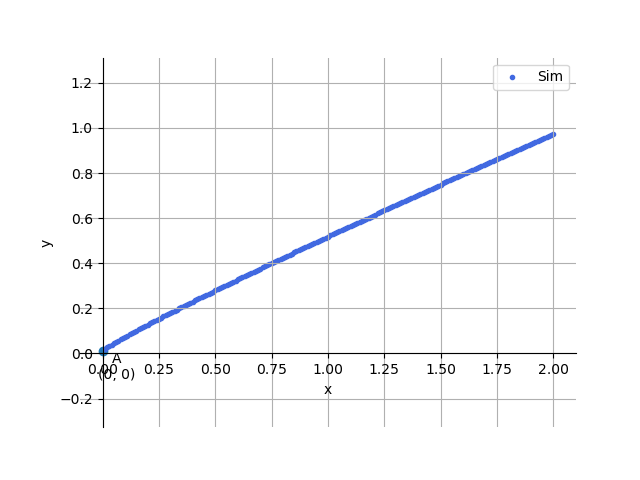
\includegraphics[width=0.7\linewidth]{figs/graph.png}
   \caption{Computational solution for $\brak{y^{\prime}}^4 + 3yy^{\prime\prime} = 0$}
\end{figure}
\end{frame}

\end{document}
